% !TeX program = pdflatex
% Heretaunga Plains Bayesian oxygen reduction: analysis record and manuscript draft
% Copyright remains with the report's author. No external data embedded.
% Compile with: pdflatex heretaunga_do_model_report.tex (twice).
% Four DO--MRT figures are exported by the active Positron R script; main text uses plots 1, 2 and 4:
%   scripts/05_DO_kinetic_trajectories and summary.R
% Run that script from the repository root to regenerate PNGs under
%   plots/final_39well/
% This .tex resolves those paths when located at the repository root or in docs/.
% The PDF is a compiled snapshot and must be recompiled after plots change.
\documentclass[11pt,a4paper]{article}
\usepackage[T1]{fontenc}
\usepackage[utf8]{inputenc}
\usepackage{lmodern}
\usepackage[margin=23mm,headheight=14pt]{geometry}
\usepackage{microtype}
\usepackage{amsmath,amssymb}
\usepackage{booktabs,tabularx,array,longtable}
\usepackage{graphicx}
\usepackage[font=small,labelfont=bf]{caption}
\usepackage{subcaption}
\usepackage{xcolor}
\usepackage{tikz}
\usetikzlibrary{arrows.meta,positioning,calc,shapes.geometric,fit,backgrounds}
\usepackage{pgfplots}
\pgfplotsset{compat=1.18}
\usepackage{enumitem}
\usepackage{fancyhdr}
\usepackage{hyperref}
\usepackage{float}
\usepackage{placeins}
\usepackage{pdflscape}
\definecolor{riverblue}{HTML}{276FBB}
\definecolor{lsrred}{HTML}{B95243}
\definecolor{aquifergreen}{HTML}{318373}
\definecolor{ink}{HTML}{182A35}
\definecolor{coolgray}{HTML}{556673}
\definecolor{pale}{HTML}{F2F5F6}
\definecolor{linegray}{HTML}{D1DCE0}
\hypersetup{colorlinks=true,linkcolor=riverblue,urlcolor=riverblue,citecolor=riverblue,pdftitle={Bayesian dissolved-oxygen reduction in the Heretaunga Plains: analysis, model selection, and interpretation}}
\setlength{\parindent}{0pt}
\setlength{\parskip}{5pt}
\setlength{\emergencystretch}{2em}
\setlist[itemize]{topsep=3pt,itemsep=2pt,leftmargin=17pt}
\setlist[enumerate]{topsep=3pt,itemsep=3pt,leftmargin=20pt}
\pagestyle{fancy}
\fancyhf{}
\fancyhead[L]{\footnotesize Heretaunga groundwater DO | Technical synthesis}
\fancyhead[R]{\footnotesize November 2026}
\fancyfoot[C]{\thepage}
\newcommand{\DO}{\mathrm{DO}}
\newcommand{\LSR}{\mathrm{LSR}}
\newcommand{\CrI}{\mathrm{CrI}}
\newcommand{\site}[1]{\texttt{#1}}
\newcommand{\mgL}{\mathrm{mg\,L^{-1}}}
\newcommand{\yr}{\mathrm{yr}}
\newcommand{\fitA}{\textsf{A: fixed river DO}}
\newcommand{\fitC}{\textsf{C: broad river DO prior}}
\newcommand{\repo}{\href{https://github.com/YugiBeer/Oxygen-Reduction-Joint-Model}{Oxygen-Reduction-Joint-Model}}
\newcommand{\plotpath}{plots/04_river_DO_prior/2801_masked_no2130/posterior_distributions/}
\newcommand{\cvplotpath}{plots/final_39well/}
% Exact PNG outputs written by scripts/05_DO_kinetic_trajectories and summary.R.
% Keep these filenames synchronised with the four save05() calls in that script.
% Main report uses plots 1, 2 and 4; plot 3 remains available for optional supplementary use.
\newcommand{\MRTplotOne}{13_DO_observed_vs_fitted_mixed_2801_masked_no2130.png}
\newcommand{\MRTplotTwo}{14_DO_river_reference_raw_samples_2801_masked_no2130.png}
\newcommand{\MRTplotThree}{15_DO_river_contribution_2801_masked_no2130.png}
\newcommand{\MRTplotFour}{16_DO_fitted_components_2801_masked_no2130.png}
% Resolve paths when this .tex is at project root OR in project docs/.
% Never point to phone-uploaded images or renamed copies in figures/.
\newcommand{\fromPlotScript}[1]{%
 \IfFileExists{plots/final_39well/#1}{%
   \includegraphics[width=.99\linewidth,height=.86\textheight,keepaspectratio]{plots/final_39well/#1}%
 }{\IfFileExists{../plots/final_39well/#1}{%
   \includegraphics[width=.99\linewidth,height=.86\textheight,keepaspectratio]{../plots/final_39well/#1}%
 }{%
   \fcolorbox{linegray}{pale}{\begin{minipage}[c][.52\textheight][c]{.88\linewidth}
   \centering\Large\textbf{Script-generated figure unavailable in this build}\par
   \vspace{8mm}\normalsize This is not a replacement image.\par
   \vspace{5mm}Run the active Positron plot script from the project root, then
   recompile the \LaTeX{} report to embed the generated output.\par
   \vspace{5mm}Expected output folder:\par
   \texttt{plots/final\_39well/}
   \end{minipage}}%
 }}%
}
\newcommand{\maybeplot}[3]{%
 \IfFileExists{#1}{%
   \begin{figure}[htbp]\centering\includegraphics[width=#2\linewidth]{#1}\caption{#3}\end{figure}%
 }{}%
}
\begin{document}
\begin{titlepage}
\vspace*{16mm}
{\Large\bfseries\color{ink} Bayesian estimation of dissolved-oxygen reduction in Heretaunga groundwater\par}
\vspace{4mm}
{\large A two-endmember mixing and dual-pathway kinetic model: workflow, validation, posterior inference, and limitations\par}
\vspace{12mm}

\begin{tikzpicture}
 \draw[riverblue,line width=2.7pt] (0,0)--(3.9,0);
 \draw[lsrred,line width=2.7pt] (4.1,0)--(7.3,0);
 \draw[aquifergreen,line width=2.7pt] (7.5,0)--(10.3,0);
\end{tikzpicture}\par
\vspace{11mm}
{\large\color{coolgray}Technical report and manuscript working draft\par}
\vspace{3mm}
\textbf{Analysis version:} regional 39-well DO likelihood, November 2026\\
\textbf{Status:} final model, grouped cross-validation and seven-fit sensitivity analysis complete; three selected DO--MRT figures (script plots 1, 2 and 4), plus a separate conceptual source-decay illustration; source-specific flowpath ages unresolved\\
\textbf{Source code:} \repo\ (script 05 exports four DO--MRT figures; the report uses plots 1, 2 and 4)\\
\textbf{Data:} local, non-public prepared groundwater dataset (not included)
\vspace{17mm}
\begin{center}
\setlength{\fboxsep}{9pt}
\fcolorbox{linegray}{pale}{%
\begin{minipage}{0.87\textwidth}
\small\textbf{Main result.} Our selected scientific model combines first-order aquifer oxygen consumption with \emph{uncertain} river-entry DO, using a truncated Normal prior centred at $7.5\,\mgL$ (SD $1.5\,\mgL$). Reanalysis of the saved posterior fit in the completed sensitivity workflow gives $k_1=0.0639\,\yr^{-1}$ (95\% credible interval $0.0458$--$0.0857$). The inferred land-surface recharge (LSR) water-table DO is $3.26\,\mgL$ (1.31--5.57). The first-order rate changes little under tested LSR saturation/prior assumptions, but more with assumed uncertainty in groundwater mean residence time (MRT). Source-specific groundwater ages remain the major structural uncertainty.
\end{minipage}}
\end{center}
\vfill
{\small\color{coolgray}Prepared for collaborator correspondence, internal technical review, and adaptation into a scientific manuscript. Numerical results derive from the final project outputs discussed in November 2026; some diagnostic plots require the user's local saved files.}\par
\end{titlepage}

\tableofcontents
\newpage

\section{Executive summary}
The aim was to identify oxygen-reduction processes in the Heretaunga groundwater system while distinguishing two potential components of dissolved-oxygen (DO) depletion: (i) reduced oxygen availability in land-surface recharge (LSR) by the time it reaches the water table, and (ii) DO consumption during subsequent aquifer residence. The analysis couples a two-endmember mixing model, informed by \(\delta^{18}\mathrm{O}\) and chloride, with alternative zero- and first-order aquifer DO kinetics and uncertain groundwater mean residence times (MRTs).

The final regional calibration contains \textbf{39 groundwater DO observations}. River-proximal site \site{2801} and the shallow, water-race-adjacent site \site{2130} are excluded from the DO likelihood, but both retain their conservative tracer observations. A separate southern outlier, \site{16758}, is removed from the prepared dataset. Four full-data model variants were fitted (two river DO assumptions by two kinetic orders), and their predictive performance was compared using five-fold grouped held-out DO cross-validation (20 additional model fits).

The final scientific interpretation adopts \textbf{first-order aquifer kinetics and an uncertain river-entry DO boundary}, with $C_R\sim\mathcal N(7.5,1.5^2)\,\mgL$ truncated to 0--14.65. Although the fixed-river first-order alternative had a small advantage in grouped CV RMSE (median $0.0342\,\mgL$), treating $7.5\,\mgL$ as an exactly known entry condition is not physically compelling. The earlier full-data summary CSV reported $k_1=0.0632\,\yr^{-1}$; the later sensitivity-run baseline (now script 06), extracted from the saved preferred CmdStanR fit, gave $k_1=0.0639\,\yr^{-1}$ (95\% CrI 0.0458--0.0857). This minor discrepancy is documented explicitly below, rather than silently combining summaries. All original full-data and sensitivity fits passed the reported MCMC checks.

Seven additional one-factor-at-a-time full-data fits examined recharge temperature (10 and $20^\circ$C), alternative LSR survival priors, and MRT log-SD (0.10 and 0.50; baseline 0.25). Estimated rate changes were under 0.2\% for temperature, $-1.0$ to $+3.4$\% for LSR prior choices, and $-4.6$ to $+18.5$\% for MRT uncertainty. The corresponding land-surface-to-water-table DO deficit is more sensitive to the assumed saturation concentration than the inferred water-table concentration.

The most important unresolved question is structural: the model estimates a separate \emph{final mixing fraction} at each well but assigns the \emph{same well-specific MRT} to river and LSR components. It therefore does not simulate distributed LSR inflow along a flowpath or the shorter residence time of recharge entering downstream. This may affect partitioning of the observed oxygen depletion between LSR entry conditions and aquifer reaction, and is a priority for scientific interpretation rather than further MCMC chain length.

Three selected script-generated DO--MRT plots (Figures~\ref{fig:mixedmrt}--\ref{fig:componentsmrt}; script plots 1, 2 and 4) distinguish \emph{observed mixed-groundwater DO}, \emph{fitted mixed-groundwater DO}, and the \emph{additive modelled river/LSR contributions}. The uncertainty whiskers represent different quantities and must not be treated as interchangeable.

\section{Research question and analysis strategy}
\subsection{Objectives}
\begin{enumerate}
\item Quantify the contribution of river recharge and land-surface recharge to sampled groundwater using conservative tracers.
\item Estimate a common aquifer DO consumption rate under zero- and first-order reaction assumptions.
\item Infer the DO of LSR reaching the water table, and the associated oxygen deficit relative to assumed DO saturation at the land surface.
\item Evaluate sensitivity to the assumed river-entry DO boundary and compare predictive skill using held-out groundwater DO measurements.
\item Test LSR saturation, oxygen-survival prior and groundwater MRT uncertainty, while distinguishing these tests from unresolved source-specific age structure.
\item Identify which estimates are supported by the observations and which depend on untested hydrogeological structure.
\end{enumerate}

\subsection{Evolution of the workflow}
The modelling programme progressed from more elaborate mixing and reaction formulations toward a parsimonious two-source framework. Earlier development considered additional mixing tracers, including sodium and excess air, paired DO--excess nitrogen formulations, and denitrification-related alternatives. Including sodium caused MCMC convergence problems, whereas excess air provided limited added value and generated conflicting results; neither is retained in the adopted tracer set. Tests of spatially varying LSR oxygen availability did not materially improve the earlier grouped CV scores (reported RMSE approximately 1.815 versus 1.812\,\(\mgL\) for common and variable LSR DO, respectively). These were \emph{developmental comparisons}, not substitutes for the final regional 39-well validation.

The final implementation retains \(\delta^{18}\mathrm{O}\) and chloride only as conservative mixing tracers, a single inferred LSR DO at the water table, and one common aquifer reaction law applied independently to each source before their contributions are mixed. This minimises unnecessary degrees of freedom while preserving uncertainty in endmember composition, source fractions, groundwater ages and rates. The Positron revisions reorganised the R scripts. The report selects three of the four DO--MRT figures generated by script 05 (plots 1, 2 and 4), directly from the saved selected first-order posterior, not by separately copying images. They illustrate different quantities rather than three independently fitted models. This PDF is a snapshot: to update it after regenerating plots, recompile the \LaTeX{} source. The conceptual source-decay figure in this report is a separate explanation. The core Stan likelihood and fitted kinetic model are unchanged.

\begin{figure}[htbp]
\centering
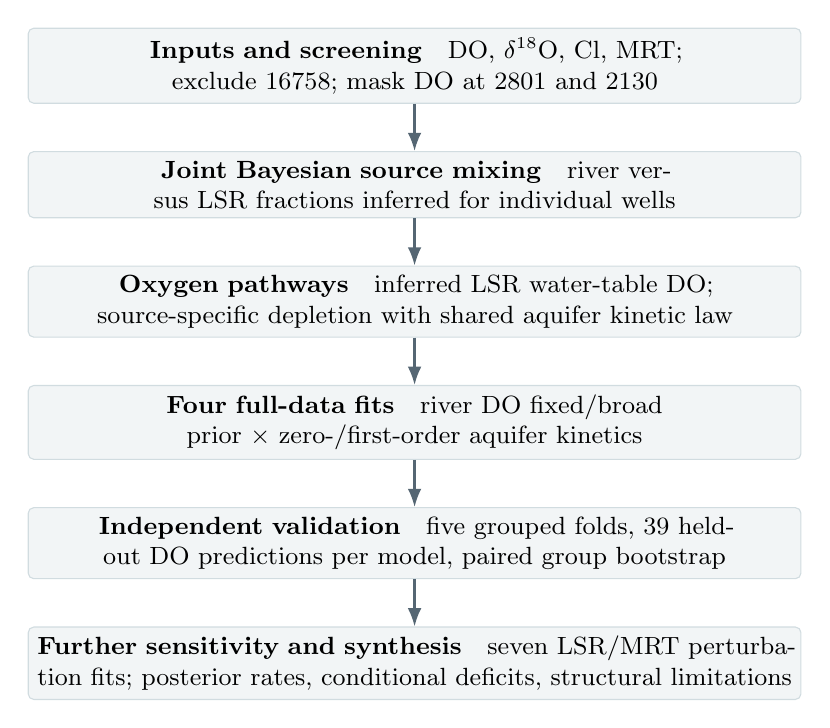
\begin{tikzpicture}[>=Latex,node distance=6mm and 9mm,
 box/.style={draw=linegray,rounded corners=2pt,fill=pale,align=center,text width=0.79\linewidth,minimum height=8mm,font=\small},
 arr/.style={-Latex,thick,draw=coolgray}]
 \node[box] (d) {\textbf{Inputs and screening}\quad DO, \(\delta^{18}\mathrm O\), Cl, MRT; exclude 16758; mask DO at 2801 and 2130};
 \node[box,below=of d] (m) {\textbf{Joint Bayesian source mixing}\quad river versus LSR fractions inferred for individual wells};
 \node[box,below=of m] (k) {\textbf{Oxygen pathways}\quad inferred LSR water-table DO; source-specific depletion with shared aquifer kinetic law};
 \node[box,below=of k] (f) {\textbf{Four full-data fits}\quad river DO fixed/broad prior \(\times\) zero-/first-order aquifer kinetics};
 \node[box,below=of f] (v) {\textbf{Independent validation}\quad five grouped folds, 39 held-out DO predictions per model, paired group bootstrap};
 \node[box,below=of v] (p) {\textbf{Further sensitivity and synthesis}\quad seven LSR/MRT perturbation fits; posterior rates, conditional deficits, structural limitations};
 \foreach \a/\b in {d/m,m/k,k/f,f/v,v/p}{\draw[arr](\a.south)--(\b.north);}
\end{tikzpicture}
\caption{Final analytical workflow. Conservative tracers remain available even when a well's DO is withheld from calibration. This diagram describes the implemented workflow, not a causal flowpath simulation.}
\label{fig:workflow}
\end{figure}

\section{Observations, screening and inclusion rules}
The private input is \texttt{data/Uwe\_HP\_data\_prepared.csv}. The fitting scripts require well identifier, depth, DO, reported MRT, \(\delta^{18}\mathrm{O}\) and chloride; they retain records with finite non-negative DO and finite non-negative reported MRT. The initial data preparation removes site \site{16758} as the identified far-south anomalous well.

After basic screening, 41 groundwater records remain, but only \textbf{39 DO responses} contribute to the final primary model:
\begin{itemize}
\item \site{2801}: measured groundwater DO \(10.2\,\mgL\), assumed MRT zero. It is river-proximal but is \emph{not} treated as a direct measurement of river-entry DO. Its actual measured DO is preserved and masked in the model likelihood.
\item \site{2130}: measured DO \(8.8\,\mgL\), reported MRT approximately 8 years. This shallow well is adjacent to a water race in the western system and may not represent regional groundwater. Its DO is excluded on a hydrogeological representativeness basis, not replaced with a modelled value.
\item At both sites, isotope and chloride data are retained for source mixing; the masking acts on the DO likelihood, not on the groundwater record as a whole.
\end{itemize}

The choice to exclude \site{2130} follows investigation of the systematic underprediction of this high-DO observation. It should be documented transparently when reporting regional inference. The previous 40-well analysis (which includes 2130 DO) remains historical sensitivity evidence, not the preferred regional calibration.

\section{Mathematical model}
\subsection{Conservative two-endmember mixing}
For each well \(i\), the inferred land-surface recharge fraction \(f_i\) is restricted to \([0,1]\), with river recharge fraction \(1-f_i\). Expected conservative tracer concentrations are
\begin{align}
 \widehat{\delta^{18}O}_i &=(1-f_i)\,\delta^{18}O_R+f_i\,\delta^{18}O_{\LSR},\\
 \widehat{\mathrm{Cl}}_i &=(1-f_i)\,\mathrm{Cl}_R+f_i\,\mathrm{Cl}_{\LSR}.\label{eq:mix}
\end{align}

Both source endmembers are estimated with informative, bounded prior distributions. The priors in the current Stan formulation have centres \(-7.79\) and \(-6.58\) per mil for river and LSR \(\delta^{18}\mathrm O\), and \(4.9\) and \(60\,\mgL\) for river and LSR chloride, respectively; corresponding prior scales are \(0.24\), \(0.40\), \(3\) and \(15\). The Stan code also constrains source ranges. Each well has an independent \(f_i\sim\mathrm{Beta}(1,1)\) prior, but \(f_i\) is estimated \emph{jointly} from its tracers and DO, not solely from conservative tracers. Isotope uncertainty includes an inferred LSR-fraction-dependent contribution, and chloride uncertainty includes a measurement-error component plus inferred residual dispersion.

An important distinction: the model permits higher \(f_i\) at greater distance from a river if the observations support it, but contains \textbf{no explicit distance-to-river covariate, monotonic mixing constraint or transport equation}. The mixing fractions describe the sampled composition of each well, not the chronology of recharge addition.

\subsection{Oxygen boundary conditions}
The assumed DO of rainfall/LSR at the land surface is freshwater saturation at \(15^{\circ}\mathrm C\), approximately \(C_{\mathrm{sat}}\simeq10\,\mgL\), assuming atmospheric pressure ratio one. A common, unknown survival fraction \(s\) determines the DO concentration where LSR enters the groundwater system:
\begin{equation}
 C_{\LSR,WT}=sC_{\mathrm{sat}},\qquad s\sim\mathrm{Beta}(1,1),\qquad
 \Delta C_{\LSR}=C_{\mathrm{sat}}-C_{\LSR,WT}.
 \label{eq:boundary}
\end{equation}
The inferred \(\Delta C_{\LSR}\) is termed the \emph{LSR oxygen deficit}. Without independent vadose residence-time information, it is \emph{not} a separate fitted vadose-zone reaction rate.

Two river-entry boundary treatments are evaluated:
\begin{align}
 \text{Scenario A:}&\quad C_R=7.5\,\mgL\quad\text{(fixed)},\\
 \text{Scenario C:}&\quad C_R\sim\mathcal N(7.5,1.5^2)\,\mgL,
 \quad0\leq C_R\leq14.65\,\mgL.
 \label{eq:riverprior}
\end{align}
The constrained upper bound allows the possibility of colder, more oxygenated river water. River-entry DO is a global boundary parameter; the model does not use well \site{2801}'s measured groundwater DO as that boundary condition.

\subsection{Aquifer oxygen consumption}
For aquifer exposure duration \(t\), the competing reaction laws are fitted \emph{separately}:
\begin{align}
 \text{Zero order:}\qquad C^{(0)}(t;C_0)&=\max(0,C_0-k_0t),
 & [k_0]&=\mgL\,\yr^{-1},\\
 \text{First order:}\qquad C^{(1)}(t;C_0)&=C_0\exp(-k_1t),
 & [k_1]&=\yr^{-1}.
 \label{eq:kinetics}
\end{align}
In the code, \(k_0=k_{\mathrm{ref}}\times7.5\,\mgL\) and \(k_1=k_{\mathrm{ref}}\); both models use the same positive reference-rate prior specification but have different physical units and kinetics. There is \emph{one} aquifer consumption rate in each model, shared between the two recharge components.

For the selected first-order form, predicted mean DO at well \(i\) is
\begin{align}
 \widehat{\DO}_i
  &=(1-f_i)C_R\exp(-k_1t_i)
    +f_iC_{\LSR,WT}\exp(-k_1t_i)\\
  &=\big[(1-f_i)C_R+f_iC_{\LSR,WT}\big]\exp(-k_1t_i).
 \label{eq:do}
\end{align}
For zero order, each source concentration is reduced with its own \(\max(0,\cdot)\) before the depleted contributions are mixed. Thus, mixing and zero-order reduction must not be interchanged algebraically without retaining the non-negativity operation.

The observed DO likelihood is Student-\(t\) with four degrees of freedom and scale \(\sqrt{0.2^2+\sigma_{\DO}^2}\,\mgL\). This allows greater robustness to outliers than a normal residual model. DO is not a conservative mixing tracer.

\subsection{Groundwater residence-time treatment}
Positive reported MRTs are treated as uncertain rather than exact:
\begin{equation}
 t_i=\exp\!\left[\log(\mathrm{MRT}_i)-\frac{\sigma_t^2}{2}
 +\sigma_tz_i\right],\qquad z_i\sim\mathcal N(0,1),\quad\sigma_t=0.25.
 \label{eq:mrt}
\end{equation}
The mean-preserving lognormal parameterisation centres the prior arithmetic mean of \(t_i\) on the reported MRT. Site \site{2801}, assigned MRT zero, has \(t=0\). Most importantly, the model assumes \textbf{the same effective aquifer residence time for both recharge sources at a given well}. This simplifying assumption is revisited in Section~\ref{sec:flowpath}.

\begin{figure}[htbp]
\centering
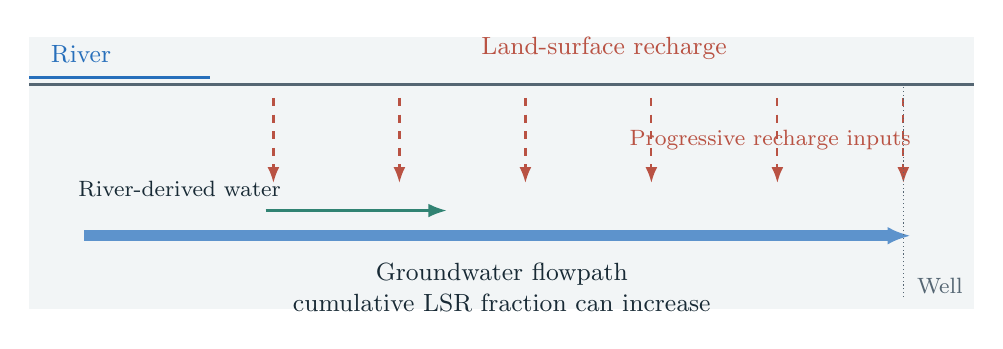
\begin{tikzpicture}[font=\small,>=Latex,scale=1]
 \fill[pale] (0,0) rectangle (12,3.45);
 \draw[thick,coolgray] (0,2.85)--(12,2.85);
 \draw[riverblue,very thick] (0,2.94)--(2.3,2.94);
 \node[anchor=south west,text=riverblue] at (.15,3.0) {River};
 \node[anchor=south,text=lsrred] at (7.3,3.05) {Land-surface recharge};
 \foreach \x in {3.1,4.7,6.3,7.9,9.5,11.1} {
   \draw[lsrred,thick,dashed,-{Latex[length=2mm]}] (\x,2.68)--(\x,1.6);
 }
 \draw[line width=4pt,riverblue!75,-{Latex[length=3mm]}] (.7,.93) -- (11.2,.93);
 \draw[aquifergreen,thick,-Latex] (3.0,1.25) -- (5.3,1.25);
 \node[anchor=north,text=ink,align=center] at (6.0,.70) {Groundwater flowpath\\cumulative LSR fraction can increase};
 \node[anchor=west,text=lsrred,font=\footnotesize] at (7.5,2.15) {Progressive recharge inputs};
 \node[anchor=south west,text=ink,font=\footnotesize] at (.5,1.3) {River-derived water};
 \draw[densely dotted,coolgray] (11.1,0.15)--(11.1,2.82);
 \node[anchor=west,text=coolgray,font=\footnotesize] at (11.15,.3) {Well};
\end{tikzpicture}
\caption{Conceptual groundwater flowpath. Increasing LSR contribution with distance can be represented by increasing well-specific \(f_i\). The time at which individual LSR increments entered the aquifer, however, is not represented by the common well-specific MRT. The drawing is conceptual, not a cross-section inferred from mapped data.}
\label{fig:flowpath}
\end{figure}

\section{Bayesian computation and diagnostics}
The model was implemented in Stan via \path{stan/04_river_DO_prior_sensitivity.stan}, called by R/CmdStanR. Four independent full-data posterior fits compare two river boundary assumptions with zero- and first-order kinetics. Each full-data model uses four chains, 1,400 warm-up and 1,400 retained sampling iterations per chain: \(5{,}600\) retained posterior draws per model. The configuration uses target acceptance \(\texttt{adapt\_delta}=0.98\) and maximum tree depth 13.

Convergence was assessed with rank-based \(\widehat R\), bulk effective sample size (ESS), divergent transitions, maximum tree-depth hits and energy-based fraction of missing information (E-BFMI). All four final full-data models passed the reported gates. Table~\ref{tab:diagnostics} reproduces the final outputs.

\begin{table}[htbp]
\centering\small
\caption{Reported full-data Stan diagnostics for the final four variants. The ESS values are the minima across parameters monitored by script 04; they are not limited to the main scientific parameters.}
\label{tab:diagnostics}
\begin{tabular}{llrrrrr}
\toprule
River boundary & Aquifer order & Max \(\widehat R\) & Min bulk ESS & Divergences & Depth hits & Min E-BFMI\\
\midrule
Fixed 7.5 & Zero & 1.01 & 713 & 0 & 0 & 0.445\\
Fixed 7.5 & First & 1.01 & 1,031 & 0 & 0 & 0.478\\
Broad prior & Zero & 1.00 & 852 & 0 & 0 & 0.444\\
Broad prior & First & 1.00 & 874 & 0 & 0 & 0.479\\
\bottomrule
\end{tabular}
\end{table}

For the fixed-boundary first-order \emph{comparator}, the key parameters had even larger bulk/tail ESS: 4,265/4,373 for the aquifer rate, 3,628/3,013 for LSR DO deficit, and 5,070/4,304 for residual DO dispersion. The associated maximum \(\widehat R\) was 1.00 to the printed precision. The resulting numerical Monte Carlo uncertainty is much smaller than parameter uncertainty; longer chains are not indicated by the available diagnostics. Convergence does not, by itself, establish the correctness of the hydrogeological model.

\section{Grouped held-out cross-validation}
\label{sec:crossvalidation}
\subsection{Design}
Cross-validation used five matched folds, retaining all observations from a named well family in the same fold where applicable. The 39 eligible DO observations are scored once per model; the four variants use identical fold assignments. For a held-out well, its DO likelihood indicator is switched off, but its tracer measurements and reported MRT remain available. Thus, the predictive assessment is \emph{held-out DO conditional on available chemistry and age information}, not prediction at a wholly unsampled location.

Four model variants across five folds result in 20 CV fits. Two fold-3 fits initially had insufficient effective sample size and were selectively resampled for more iterations; the completed set passed the CV diagnostics and supported grouped bootstrap comparison. A paired bootstrap resamples the prespecified well groups, not independent posterior observations, and compares RMSE or MAE for the same held-out well set. The reported 95\% bootstrap intervals quantify variability of the paired prediction metrics under this grouping and are not posterior credible intervals for a kinetic coefficient.

\subsection{Paired results}
Let \(\Delta\mathrm{RMSE}=\mathrm{RMSE}(\mathrm{candidate})-\mathrm{RMSE}(\mathrm{comparator})\). Negative values favour the candidate. Table~\ref{tab:cv} and Figure~\ref{fig:cvforest} summarise the completed paired bootstrap results.

\begin{table}[htbp]
\centering\small
\caption{Paired grouped-bootstrap predictive differences (\(\mgL\)); intervals are 2.5th--97.5th percentiles. Negative candidate-minus-comparator values favour the candidate.}
\label{tab:cv}
\begin{tabularx}{\linewidth}{>{\raggedright\arraybackslash}Xrr}
\toprule
Candidate minus comparator & Median \(\Delta\mathrm{RMSE}\) [95\% interval] & Median \(\Delta\mathrm{MAE}\) [95\% interval]\\
\midrule
Broad minus fixed (first order) & \phantom{-}0.0342 [0.00564, 0.0751] & \phantom{-}0.0204 [-0.00873, 0.0664]\\
Broad minus fixed (zero order) & -0.0482 [-0.132, 0.0480] & -0.0555 [-0.145, 0.0323]\\
First minus zero (broad river prior) & -0.0473 [-0.133, 0.0321] & \phantom{-}0.0192 [-0.0553, 0.0818]\\
First minus zero (fixed river DO) & \textbf{-0.132 [-0.238, -0.0126]} & -0.0593 [-0.162, 0.0265]\\
\bottomrule
\end{tabularx}
\end{table}

\begin{figure}[htbp]
\centering
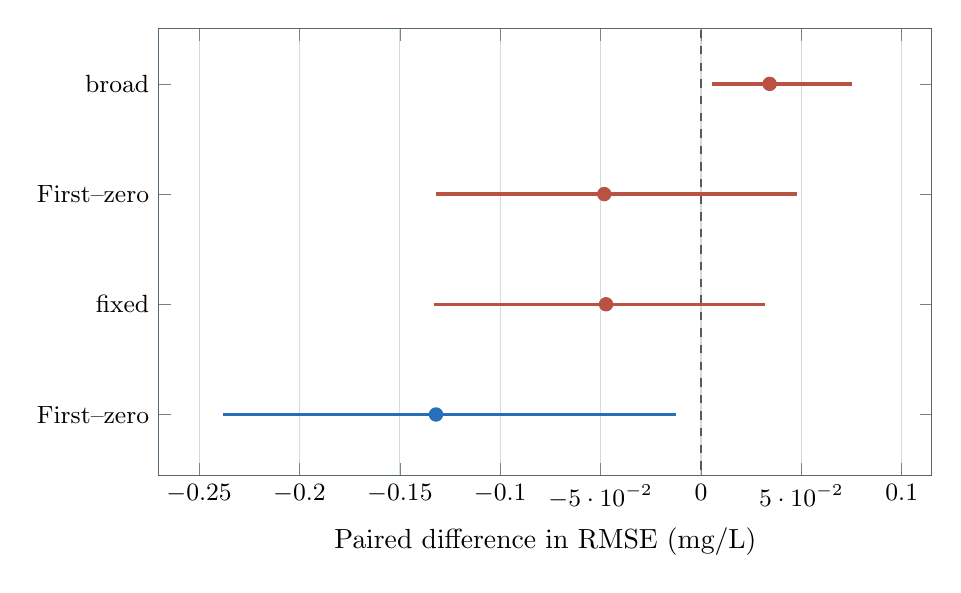
\begin{tikzpicture}
\begin{axis}[
 width=.94\linewidth,height=7.25cm,
 xmin=-0.27,xmax=0.115,ymin=.45,ymax=4.5,
 ytick={1,2,3,4},
 yticklabels={First--zero, fixed,First--zero, broad,Broad--fixed, zero,Broad--fixed, first},
 xmajorgrids=true,grid style={linegray},
 xlabel={Paired difference in RMSE (mg/L)},
 yticklabel style={font=\small,align=right},
 tick label style={font=\small},
 axis line style={coolgray},
 enlarge y limits=false,
 clip=false
]
 \addplot[dashed,black!65,thick] coordinates {(0,.5) (0,4.5)};
 \addplot[riverblue,very thick] coordinates {(-.238,1) (-.0126,1)};
 \addplot[riverblue,only marks,mark=*,mark size=2.4pt] coordinates {(-.132,1)};
 \addplot[lsrred,very thick] coordinates {(-.133,2) (.0321,2)};
 \addplot[lsrred,only marks,mark=*,mark size=2.4pt] coordinates {(-.0473,2)};
 \addplot[lsrred,very thick] coordinates {(-.132,3) (.048,3)};
 \addplot[lsrred,only marks,mark=*,mark size=2.4pt] coordinates {(-.0482,3)};
 \addplot[lsrred,very thick] coordinates {(.00564,4) (.0751,4)};
 \addplot[lsrred,only marks,mark=*,mark size=2.4pt] coordinates {(.0342,4)};
\end{axis}
\end{tikzpicture}
\caption{Median differences in held-out RMSE and grouped-bootstrap 95\% intervals. A negative difference indicates lower prediction error for the candidate model. The fixed-river, first-order formulation performs better than fixed-river zero-order by RMSE under this validation design, while other differences are generally small and/or less conclusive.}
\label{fig:cvforest}
\end{figure}

The fixed-river first-order model improves RMSE relative to fixed-river zero-order by a median \(0.132\,\mgL\), with a paired 95\% interval that excludes zero. The corresponding MAE interval includes zero; the result should therefore not be presented as a large or unequivocal performance gain. Under first-order kinetics, widening the river DO boundary to the broad prior slightly \emph{worsens} RMSE (median \(+0.0342\,\mgL\)). For \emph{predictive RMSE alone}, the fixed-river first-order option is marginally better. For \emph{scientific interpretation}, we select the uncertain-river first-order option because a fixed $7.5\,\mgL$ entry boundary would treat a variable physical quantity as perfectly known. In the broad-river comparison, first-minus-zero order improves median RMSE by $0.0473\,\mgL$, but the paired interval includes zero; hence preference for first-order kinetics is not statistically decisive under every boundary assumption. Absolute 39-well CV scores should be read from the corresponding final \texttt{cv\_scores.csv} before submitting a paper; they are not reproduced here because that final file was not supplied for this synthesis.

\FloatBarrier
\section{Final posterior parameter estimates}
Table~\ref{tab:parameters} shows the fitted full-data posterior medians and central 95\% credible intervals for all four variants. Rate units differ between kinetic orders and should not be compared as though they were the same physical quantity.

\begin{table}[htbp]
\centering\footnotesize
\caption{Earlier full-data posterior CSV summaries (before the later sensitivity-run saved-fit re-summarisation), medians with 95\% credible intervals. River and LSR DO units are $\mgL$; zero-order rates are $\mgL\,\yr^{-1}$ and first-order rates are $\yr^{-1}$. The broad-river first-order fit is the scientific primary.}
\label{tab:parameters}
\resizebox{\linewidth}{!}{%
\begin{tabular}{llrrrr}
\toprule
Boundary & Order & River-entry DO & Aquifer rate & LSR DO at WT & LSR DO deficit\\
\midrule
Fixed & Zero & 7.50 (fixed) & 0.235 [0.189, 0.293] & 3.62 [0.462, 5.45] & 6.38 [4.55, 9.54]\\
Fixed & First & 7.50 (fixed) & 0.0625 [0.0484, 0.0812] & 3.28 [1.42, 5.47] & 6.72 [4.53, 8.58]\\
Broad & Zero & 6.35 [5.02, 8.47] & 0.188 [0.125, 0.294] & 3.98 [0.825, 5.43] & 6.02 [4.57, 9.18]\\
\textbf{Broad} & \textbf{First} & \textbf{7.66 [5.75, 9.74]} & \textbf{0.0632 [0.0453, 0.0851]} & \textbf{3.21 [1.25, 5.55]} & \textbf{6.79 [4.45, 8.75]}\\
\bottomrule
\end{tabular}}
\end{table}

\subsection{Selected first-order solution and posterior consistency}
The scientific primary has an uncertain river-entry DO boundary. The \emph{later baseline} from the sensitivity workflow (current script 06), which reads the preferred posterior fit originally saved by current script 02, gives
\begin{equation}
 \boxed{k_1=0.0639\,\yr^{-1}\quad(95\%\ \CrI:\ 0.0458\text{--}0.0857\,\yr^{-1}).}
\end{equation}
Its corresponding LSR water-table DO is $3.26\,\mgL$ (95\% CrI 1.31--5.57) and its LSR DO deficit is $6.78\,\mgL$ (4.46--8.72). The effective first-order half-life at the posterior median is $\ln(2)/k_1\simeq10.8$ years; this is a kinetic interpretation, not a measured groundwater transit time.

\textbf{Consistency note.} The earlier full-data summary CSV (Table~\ref{tab:parameters}) reported $k_1=0.0632$ (0.0453--0.0851), LSR water-table DO 3.21 (1.25--5.55) and deficit 6.79 (4.45--8.75). The sensitivity-run baseline reported $0.0639$, 3.26 and 6.78 from the saved fit. These differences are small but need provenance reconciliation before formal publication. The renumbered script 04 reads the preferred RDS directly and warns when its rate disagrees with the earlier summary CSV; the new script 05 independently prints a four-parameter summary from the same saved RDS. The previously reported broad-boundary river DO posterior is 7.66 (5.75--9.74) $\mgL$, which has not been independently re-summarised for the present report.

The LSR deficit is the \emph{difference between assumed surface DO and inferred water-table DO}. It is a model-conditional concentration deficit, not a measured vadose-zone oxygen consumption rate or proof of where the oxygen was removed.

\begin{figure}[htbp]
\centering
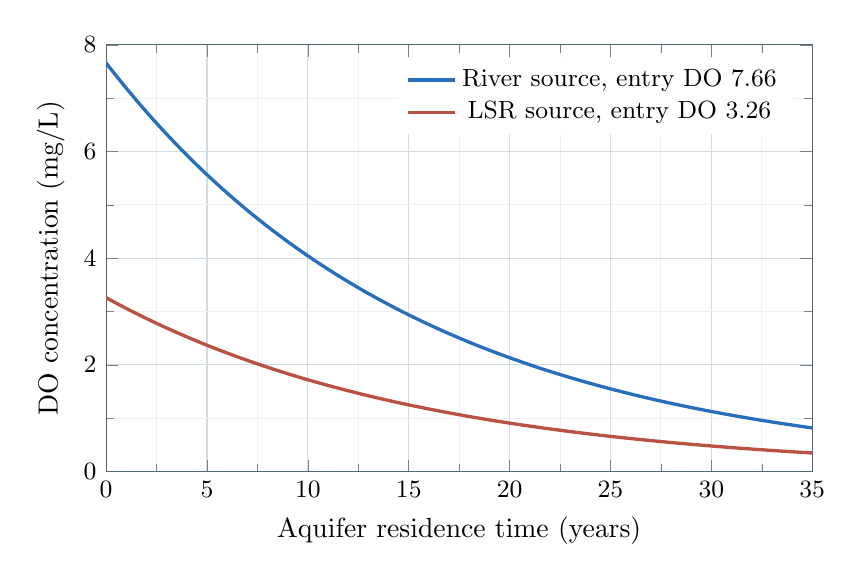
\begin{tikzpicture}
\begin{axis}[
 width=.87\linewidth,height=7.0cm,
 xmin=0,xmax=35,ymin=0,ymax=8.0,
 xlabel={Aquifer residence time (years)},ylabel={DO concentration (mg/L)},
 grid=both,minor tick num=1,major grid style={linegray},
 minor grid style={linegray!40},
 legend style={draw=none,fill=white,font=\small,at={(.97,.97)},anchor=north east},
 tick label style={font=\small},axis line style={coolgray}
]
 \addplot[riverblue,very thick,domain=0:35,samples=90] {7.66*exp(-0.0639*x)};
 \addlegendentry{River source, entry DO 7.66}
 \addplot[lsrred,very thick,domain=0:35,samples=90] {3.26*exp(-0.0639*x)};
 \addlegendentry{LSR source, entry DO 3.26}
\end{axis}
\end{tikzpicture}
\caption{Illustrative first-order DO decay using the \emph{later reported} median rate $0.0639\,\yr^{-1}$ and input DO medians for the uncertain river-boundary model. The curves show model behaviour for isolated source components; they are not observed concentration transects, not posterior credible bands, and do not represent progressively added LSR.}
\label{fig:decay}
\end{figure}

\subsection{Three selected DO--MRT plots: observed concentrations, river reference and source contributions}
\label{sec:threeplots}
The active \path{scripts/05_DO_kinetic_trajectories and summary.R} exports \emph{four} complementary DO--MRT PNG files under \path{plots/final_39well/}. The report deliberately uses \textbf{script Plots 1, 2 and 4}. The original Plot 3 (river-derived share versus an unweighted 100\%-river reference) is still generated but not shown here, because the comparison of a weighted source contribution with a pure-source concentration can be misread as evidence of model misfit. All selected figures derive from the same preferred first-order posterior; there is no additional model fitting.

\begin{enumerate}[leftmargin=17pt,itemsep=4pt]
\item \textbf{Plot 1: observed versus fitted mixed-groundwater DO (Figure~\ref{fig:mixedmrt}).} Open black circles show DO measured at sites included in the model likelihood; crosses identify observations excluded from it. Sites \site{2801} (measured DO 10.2\,mg/L; nominal MRT 0) and \site{2130} (8.8\,mg/L) are excluded from the DO likelihood but remain labelled. Coloured points are the posterior \emph{medians} of well-specific fitted mixed-groundwater DO, with colour denoting inferred LSR fraction. The whiskers are 95\% \emph{posterior predictive intervals} based on replicated DO, which include the model's observation-level residual variability. This is the direct comparison of the modelled and observed mixed samples.
\item \textbf{Plot 2: raw measured mixed-sample DO versus a 100\%-river reference (Figure~\ref{fig:samplemrt}).} The sample points show \emph{raw measured DO}; the dashed line and blue ribbon are the posterior median and 95\% credible interval of the first-order river-only DO trajectory. As the groundwater samples contain variable LSR fractions, this river-only band is \emph{not} a prediction interval for observed mixed-groundwater DO. Sample observations below the curve do not, by themselves, demonstrate poor model fit.
\item \textbf{Plot 4: fitted river and LSR DO contributions (Figure~\ref{fig:componentsmrt}).} The vertical blue and red segments give the \emph{river-derived} and \emph{LSR-derived} parts of the modelled DO concentration in each mixed sample. At each posterior draw, the two source contributions obey
\begin{align}
 C_{R,i} &= (1-f_i)\,C_{R,\mathrm{entry}}\exp(-k_1t_i),\\
 C_{\LSR,i} &= f_i\,C_{\LSR,\mathrm{WT}}\exp(-k_1t_i),\\
 \mu_i &= C_{R,i}+C_{\LSR,i},
\end{align}
where $f_i$ is the inferred LSR fraction and $t_i$ is the assumed shared aquifer residence time. The stacked blue and red segment heights are \emph{posterior means}, not posterior medians. This is intentional: $\mathbb{E}[C_{R,i}]+\mathbb{E}[C_{\LSR,i}]=\mathbb{E}[\mu_i]$, so the stacked total matches the black fitted-total point exactly. Open circles and crosses show the \emph{observed} sample DO, and grey whiskers give 95\% \emph{credible intervals for the fitted mean DO}, not posterior predictive intervals for a new observation. This panel shows how the two pathways combine to produce the fitted DO, and how their sum compares with measurement.
\end{enumerate}

The selected figures therefore serve different purposes: Figure~\ref{fig:mixedmrt} assesses sample-level fit including predictive uncertainty; Figure~\ref{fig:samplemrt} illustrates the river-only kinetic reference against raw mixed samples; and Figure~\ref{fig:componentsmrt} decomposes the \emph{fitted mixed-sample DO} into two source components. None is independent validation of the model; predictive validation comes from grouped held-out cross-validation (Section~\ref{sec:crossvalidation}). The source decomposition remains conditional on the model's assumption that river and LSR components share the same well-specific MRT.

\textbf{Figure provenance.} Each displayed panel is linked to the PNG filename written by script 05 under \path{plots/final_39well/}: outputs 13, 14 and 16. Plot 3 (output 15) remains a script-generated diagnostic but is omitted from the main report. No phone-uploaded screenshots are embedded. The present PDF uses explicit missing-output notices wherever a local script-generated PNG is unavailable; regenerating the images in Positron and recompiling this \LaTeX{} file inserts the current figure outputs.

\clearpage
\begin{landscape}
\begin{figure}[H]
\centering
\fromPlotScript{\MRTplotOne}
\caption{\textbf{Observed and model-fitted groundwater DO.} Open circles and crosses: measured mixed-sample DO (\site{2801} and \site{2130} are excluded from the DO likelihood; the script displays 2801's original 10.2\,mg/L observation). Coloured points: sample-specific posterior median fitted mixed-groundwater DO; colour represents the inferred LSR fraction. Vertical whiskers: 95\% in-sample posterior predictive intervals, including observation variability. This figure provides the direct sample-level fitted-versus-observed assessment, not a river-endmember comparison.}
\label{fig:mixedmrt}
\end{figure}
\end{landscape}
\clearpage
\begin{landscape}
\begin{figure}[H]
\centering
\fromPlotScript{\MRTplotTwo}
\caption{\textbf{Measured mixed-groundwater DO versus the first-order river-only reference.} Coloured markers: observed groundwater DO concentrations and inferred LSR fraction. Dashed black curve and light-blue band: posterior median and 95\% credible interval for a hypothetical 100\%-river-derived groundwater component versus MRT. These are \emph{not} limits for the observed mixed samples: LSR inputs alter the sample DO, so many points can lie below the river-only trajectory without contradicting the fitted model. The script plots all retained original DO observations, including \site{2801} at 10.2\,mg/L, without a restrictive 10\,mg/L y-axis maximum.}
\label{fig:samplemrt}
\end{figure}
\end{landscape}
\clearpage
\begin{landscape}
\begin{figure}[H]
\centering
\fromPlotScript{\MRTplotFour}
\caption{\textbf{Additive fitted river and LSR contributions to mixed-groundwater DO (script Plot 4).} Blue and red vertical segments are the posterior \emph{mean} river-derived and LSR-derived DO contributions, respectively, each in mg/L of the final mixed sample. Their stacked sum is the fitted total DO (black point). Open circles and crosses show measured DO included in or excluded from the likelihood, respectively. Grey whiskers are 95\% posterior \emph{credible intervals for the fitted mean DO}; unlike Figure~\ref{fig:mixedmrt}, they do not include observation-level posterior predictive dispersion. The source split is a model-based inference and is not an independent validation of the assumed common MRT.}
\label{fig:componentsmrt}
\end{figure}
\end{landscape}
\clearpage

The separate conceptual first-order source-decay illustration (Figure~\ref{fig:decay}) explains the reaction law but is \emph{not} one of the three displayed DO--MRT plots. Script Plot 3 remains available as an optional diagnostic and is not included here. The preferred-fit posterior summary from script 05 is likewise distinct; the previously noted $0.0632$ versus $0.0639\,\yr^{-1}$ rate-summary discrepancy still requires reconciliation with the saved draws before formal publication.

\subsection{Boundary sensitivity and posterior dependence}
The first-order rate changes little between the fixed boundary and the initially reported uncertain-river fit (0.0625 versus $0.0632\,\yr^{-1}$); the later saved-fit baseline was $0.0639\,\yr^{-1}$. LSR water-table DO and deficit also remain similar at the posterior median. This is evidence of stability \emph{within the tested family of models}, not proof of independence from all river-water oxygen dynamics.

The fixed-river first-order comparator has a posterior correlation of approximately $-0.397$ between LSR oxygen deficit and aquifer rate, while the selected broad-river first-order formulation has a smaller negative correlation (approximately $-0.192$). The sign is physically coherent: greater DO loss before aquifer entry can, to some extent, be offset by slower aquifer reduction. In the broad-river sensitivity, river DO and aquifer rate are correlated positively (\(+0.838\) for zero-order; \(+0.544\) for first-order), indicating appreciable parameter compensation when the input DO is not fixed. The smaller first-order correlation is consistent with less river-boundary/rate confounding in that formulation.

\begin{table}[htbp]
\centering\small
\caption{Posterior pairwise correlations from the four full-data models. N/A denotes a fixed river DO, for which correlation with its constant value is undefined.}
\label{tab:corr}
\begin{tabular}{llrrr}
\toprule
River boundary & Order & River DO vs rate & River DO vs LSR deficit & LSR deficit vs rate\\
\midrule
Fixed & Zero & N/A & N/A & -0.181\\
Fixed & First & N/A & N/A & -0.397\\
Broad & Zero & 0.838 & 0.404 & 0.175\\
Broad & First & 0.544 & 0.281 & -0.192\\
\bottomrule
\end{tabular}
\end{table}


\FloatBarrier
\section{Completed sensitivity to LSR boundary and MRT uncertainty}
\label{sec:sensitivity}
Seven one-factor-at-a-time modifications of the selected \emph{uncertain-river, first-order} model were fitted using the same 39 DO-likelihood wells. The reference case is recharge saturation at $15^\circ$C, an LSR oxygen survival prior $s\sim\mathrm{Beta}(1,1)$, and age log-SD $\sigma_t=0.25$. The river DO prior and aquifer reaction law remain unchanged throughout. These are \emph{conditional model sensitivity tests}; they are not source-specific transit-time models or further held-out predictive comparisons.

\begin{table}[htbp]
\centering\footnotesize
\caption{Completed script-07 sensitivity analysis, from the user's reported output files. The percentages are relative to the \emph{saved-fit} baseline median $0.0639\,\yr^{-1}$. All eight fits passed the script-07 MCMC gates. Concentration medians are in $\mgL$.}
\label{tab:sen}
\resizebox{\linewidth}{!}{%
\begin{tabular}{lrrrrr}
\toprule
Scenario & Median $k_1$ [$\yr^{-1}$] & 95\% CrI & Change [\%] & LSR WT DO & LSR deficit\\
\midrule
Baseline: $15^\circ$C; Beta(1,1); MRT SD 0.25 & 0.0639 & [0.0458,0.0857] & 0.00 & 3.26 & 6.78\\
LSR saturation $10^\circ$C & 0.0638 & [0.0462,0.0854] & -0.120 & 3.25 & 8.02\\
LSR saturation $20^\circ$C & 0.0639 & [0.0459,0.0862] & +0.036 & 3.23 & 5.79\\
LSR survival Beta(2,2) & 0.0638 & [0.0458,0.0860] & -0.032 & 3.42 & 6.61\\
LSR survival Beta(2,5) & 0.0632 & [0.0451,0.0845] & -0.997 & 3.01 & 7.03\\
LSR survival Beta(5,2) & 0.0660 & [0.0479,0.0887] & +3.38 & 4.28 & 5.75\\
MRT log-SD 0.10 & 0.0610 & [0.0448,0.0797] & -4.55 & 3.13 & 6.91\\
MRT log-SD 0.50 & 0.0757 & [0.0520,0.108] & +18.5 & 3.90 & 6.13\\
\bottomrule
\end{tabular}}
\end{table}

\begin{figure}[htbp]
\centering
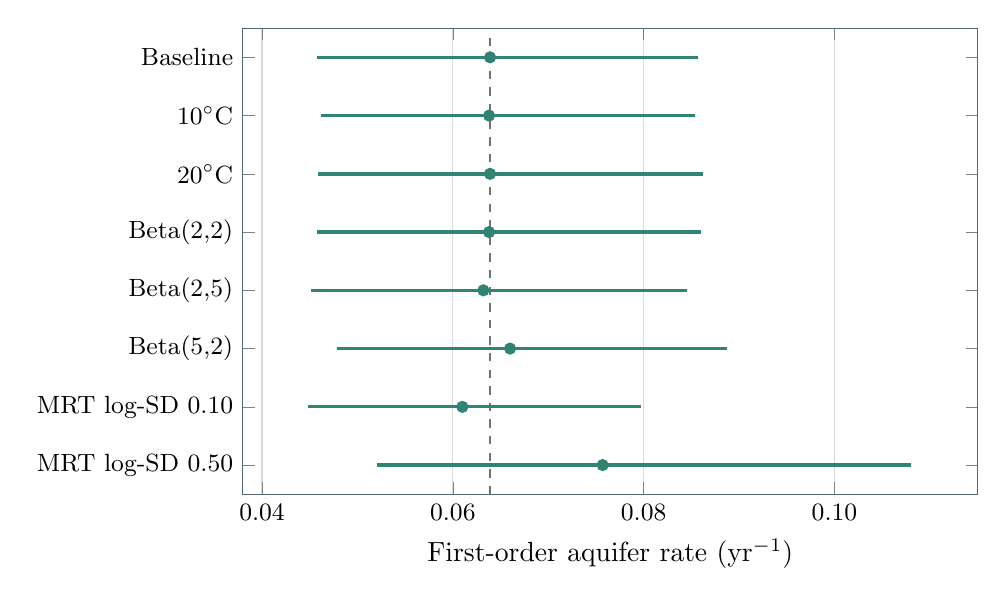
\begin{tikzpicture}
\begin{axis}[
 width=.90\linewidth,height=7.5cm,
 xmin=.038,xmax=.115,ymin=.5,ymax=8.5,
 xtick={0.04,0.06,0.08,0.10},
 xticklabels={0.04,0.06,0.08,0.10},
 xticklabel style={font=\small},
 ytick={1,2,3,4,5,6,7,8},
 yticklabels={{MRT log-SD 0.50},{MRT log-SD 0.10},{Beta(5,2)},{Beta(2,5)},{Beta(2,2)},{20$^\circ$C},{10$^\circ$C},{Baseline}},
 yticklabel style={font=\small,align=right},tick label style={font=\small},
 xlabel={First-order aquifer rate (yr$^{-1}$)},
 xmajorgrids=true,grid style={linegray},axis line style={coolgray},clip=false
 ]
 \addplot[dashed,black!55] coordinates {(.0639,.5)(.0639,8.5)};
 \foreach \low/\high/\med/\y in {
 .0520/.108/.0757/1,
 .0448/.0797/.0610/2,
 .0479/.0887/.0660/3,
 .0451/.0845/.0632/4,
 .0458/.0860/.0638/5,
 .0459/.0862/.0639/6,
 .0462/.0854/.0638/7,
 .0458/.0857/.0639/8
 } {
 \addplot[aquifergreen,very thick] coordinates {(\low,\y)(\high,\y)};
 \addplot[aquifergreen,only marks,mark=*,mark size=2pt] coordinates {(\med,\y)};
 }
\end{axis}
\end{tikzpicture}
\caption{First-order rate posterior medians and 95\% credible intervals for alternative assumptions. The dashed line marks the baseline median. These are \emph{within-model} intervals, not intervals for scenario differences.}
\label{fig:sensitivity}
\end{figure}

Temperature changes from 10 to $20^\circ$C alter the median rate by less than 0.2\%; alternative LSR survival priors alter it by approximately $-1.0$ to $+3.4$\%. Water-table LSR DO remains near $3.2$--$3.3\,\mgL$ across the temperature scenarios, whereas the surface-to-water-table oxygen deficit shifts from $8.02$ to $5.79\,\mgL$. This is partly a consequence of the \emph{definition} of the deficit relative to an assumed saturation value. The prior Beta(5,2), favouring higher DO survival, shifts water-table DO to $4.28\,\mgL$, illustrating residual prior dependence.

Altering the \emph{breadth of MRT uncertainty} has the largest effect on the median rate among these tests: reducing log-SD to 0.10 lowers $k_1$ by 4.55\%, while increasing it to 0.50 raises $k_1$ by 18.5\%. These changes do not demonstrate the effect of systematically longer or shorter groundwater ages. All eight baseline/sensitivity fits passed reported convergence checks (maximum $\widehat R=1.01$, no divergent transitions or tree-depth hits, minimum E-BFMI 0.460 and minimum tail ESS 669). These checks establish numerical convergence, not hydrogeological validity.

\textbf{Interpretation:} the fitted first-order reaction rate is comparatively robust to the tested LSR saturation and survival-prior assumptions, but more sensitive to assumptions about uncertainty in groundwater ages. The tests do \emph{not} address the more fundamental uncertainty in the source-specific residence times or progressive introduction of LSR along groundwater flowpaths.

\FloatBarrier
\section{Key hydrogeological limitation: progressive addition of LSR}
\label{sec:flowpath}
\subsection{What the mixing model captures}
An increasing LSR contribution with river distance or along a downgradient groundwater flowpath is physically plausible in a system receiving diffuse land-surface recharge. The current mixing formulation, Equation~\eqref{eq:mix}, allows well-specific fractions \(f_i\) to vary from river-dominated values toward LSR-dominated values. Consequently, an increasing tracer-inferred LSR fraction along a sampled transect \emph{can be reflected in the model}. However, it is not guaranteed: neither measured river distance nor a monotonic relationship with MRT is directly included.

Because DO is part of the joint likelihood, \(f_i\) is additionally informed by the reactive observations. It is therefore best described as a \emph{jointly inferred source fraction constrained by isotope, chloride and DO data}, rather than as a wholly independent conservative tracer mixing estimate.

\subsection{What the model omits}
The present first-order DO equation (Equation~\eqref{eq:do}) implicitly assumes \(t_{R,i}=t_{\LSR,i}=t_i\). It calculates the age-reduced DO of \emph{both} source endmembers over the same duration and mixes them only at the end. In a physically distributed recharge system, some LSR may have entered the aquifer close to the sampled well, while river-derived groundwater may have experienced a much longer journey. Assigning a full river-component MRT to young LSR would tend to give that LSR excess reaction exposure; whether the fitted $k$ is biased upward or downward depends on which source the observed bulk MRT represents, their relative DO, and the fitted mixing fractions. A more flexible, still lumped representation would be
\begin{equation}
 \widehat{\DO}_i=(1-f_i)C_R\exp(-kt_{R,i})
 +f_iC_{\LSR,WT}\exp(-kt_{\LSR,i}),
 \qquad t_{R,i}\ne t_{\LSR,i}\ \text{in general}.
 \label{eq:twoages}
\end{equation}
For distributed recharge with an age spectrum, the more appropriate expression averages the exponential survival over a source-dependent travel-time distribution:
\begin{equation}
 \widehat{\DO}_i=(1-f_i)C_R\!\int_0^\infty e^{-kt}\,g_{R,i}(t)\,dt
 +f_iC_{\LSR,WT}\!\int_0^\infty e^{-kt}\,g_{\LSR,i}(t)\,dt.
 \label{eq:agedist}
\end{equation}
Here \(g_{R,i}\) and \(g_{\LSR,i}\) are source-conditioned groundwater age distributions, not quantities currently estimated in Stan. Equations~\eqref{eq:twoages} and~\eqref{eq:agedist} are conceptual extensions, \textbf{not fitted or validated results}. An observed bulk MRT cannot generally identify both component-specific travel-time distributions.

The impact on inferred rate and LSR boundary DO is not known a priori. Depending on relative source DO concentrations, recharge ages and mixing fractions, accounting for younger LSR may redistribute the inferred oxygen deficit between LSR entry conditions and subsequent aquifer reduction. It would be premature to assert the direction or magnitude of that bias without a sensitivity calculation.

\subsection{Suggested verification before manuscript submission}
\begin{enumerate}
\item Map or plot posterior \(f_i\) against \emph{measured} distance from the river, depth and reported MRT, with credible intervals. Do not treat MRT itself as a direct surrogate for distance unless demonstrated. The current input script does not provide river-distance variables to Stan; these would be joined separately from well coordinates.
\item Use existing posterior median parameters for a \emph{forward, no-refit} sensitivity calculation allowing \(t_{\LSR,i}<t_{R,i}\), under transparent scenarios. Report effects on predicted DO and whether the conclusions about k and boundary deficit are robust. This is a diagnostic, not a new calibrated result.
\item If sensitivity is substantial, seek independent constraints on source-specific ages or distributed recharge. Adding unconstrained age parameters to the present Bayesian model would risk losing the identifiability gained through parsimony.
\end{enumerate}

\section{Interpretation, strengths and limitations}
\subsection{What is supported}
\begin{itemize}
\item The selected broad-river, first-order model estimates an effective aquifer DO depletion rate with a posterior interval that excludes zero in the stated formulation. The rate is stable under the tested river and LSR boundary conditions; its sensitivity to assumed MRT uncertainty is appreciably larger.
\item The model requires substantially lower average LSR DO at aquifer entry than the assumed land-surface saturation concentration, conditional on the chosen two-source structure, residence-time model and shared LSR DO boundary.
\item Grouped held-out validation favours first-order over zero-order kinetics under the fixed-river boundary, while the first-versus-zero advantage is less conclusive under the broad boundary. The broad river DO prior has a small CV RMSE penalty versus fixed DO, but is preferable as a physically honest boundary assumption.
\item MCMC convergence is satisfactory for all four final full-data models; extending chains would not meaningfully address the dominant hydrogeological uncertainty.
\end{itemize}

\subsection{What should not be overclaimed}
\begin{itemize}
\item The inferred LSR DO deficit does not uniquely identify oxygen loss in the unsaturated zone. It is an effective difference between assumed rainfall DO and inferred water-table DO, conditional on the model.
\item The fitted rate is an effective regional kinetic parameter. It need not be constant along individual aquifer flowpaths, across redox facies or between river-derived and LSR-derived waters.
\item The model does not currently constrain source-specific ages or spatial recharge histories; increasing LSR fraction is not equivalent to progressive source addition in a reactive-transport calculation.
\item DO predictions were held out \emph{conditional on well tracer and MRT information}, not independently tested at new groundwater locations without those observations.
\item Posterior means of losses across sampled wells are not flow-weighted or aquifer-wide oxygen mass budgets.
\end{itemize}

\section{Potential manuscript wording}
\subsection*{Methods paragraph (draft)}
We implemented a joint Bayesian two-endmember mixing and dissolved-oxygen consumption model for Heretaunga groundwater. River recharge and land-surface recharge (LSR) fractions were estimated at individual wells using $\delta^{18}$O and chloride, with DO observations contributing to the joint inference. River-entry DO was assigned a truncated Normal(7.5,1.5$^2$) mg\,L$^{-1}$ prior in the selected first-order model; a fixed 7.5\,mg\,L$^{-1}$ boundary was retained for comparison. The DO of LSR reaching the water table was inferred relative to assumed freshwater saturation at the land surface (baseline 15$^\circ$C). Both sources were exposed to the same well-specific effective MRT and one aquifer reaction law, with zero- and first-order kinetics fitted separately. DO at sites 2801 and 2130 was withheld but their conservative tracers retained, leaving 39 fitted DO observations after excluding site 16758. Four full-data models were compared using matched five-fold grouped cross-validation with held-out DO; a further seven full-data sensitivity fits varied LSR saturation temperature, LSR-survival priors and age uncertainty.

\subsection*{Results paragraph (draft)}
The selected model used first-order aquifer oxygen consumption with uncertain river-entry DO. The subsequently reported saved-fit posterior median rate was $0.0639\,\yr^{-1}$ (95\% credible interval 0.0458--0.0857); inferred LSR DO at the water table was $3.26\,\mgL$ (1.31--5.57), corresponding to an LSR oxygen deficit of $6.78\,\mgL$ (4.46--8.72). An earlier summary CSV of the same model family reported a rate of $0.0632\,\yr^{-1}$ and should be reconciled with the saved posterior before publication. In grouped five-fold CV, the fixed-boundary first-order model marginally outperformed its uncertain-boundary counterpart by a median paired RMSE difference of $0.0342\,\mgL$; this small predictive difference did not justify treating river-entry DO as exactly known. A seven-fit sensitivity analysis found first-order rate changes below 0.2\% for 10--20$^\circ$C LSR saturation, $-1.0$ to $+3.4$\% for alternative LSR survival priors, and $-4.6$ to $+18.5$\% for changes in MRT log-SD from 0.25 to 0.10 or 0.50. All sensitivity fits passed reported MCMC checks. Results remain conditional on common LSR boundary DO and simplified source age representation.

\subsection*{Discussion paragraph (draft)}
The comparatively stable first-order rate under LSR boundary perturbations suggests that an effective aquifer oxygen-consumption parameter is estimable under the adopted tracer-constrained recharge model; the marked response to MRT uncertainty and unknown source-conditioned ages restricts physical interpretation. By contrast, the partition between LSR entry oxygen deficit and aquifer depletion may be more structurally sensitive. The mixing model permits increasing LSR contributions across groundwater wells but does not explicitly represent distributed recharge inputs or different residence times for river and LSR components. Because the model applies a common well-specific MRT to both source waters, the inferred LSR water-table DO is best interpreted as an effective boundary concentration, not a uniquely identified measure of oxygen consumption in the vadose zone. Future work should assess observed spatial trends in recharge fractions and the sensitivity of the fitted DO predictions to source-specific travel-time distributions.

\section{Reproducibility and figure use}
The final scripts are maintained in \repo. Following the Positron renumbering, the active workflow is:
\begin{enumerate}[leftmargin=14pt,itemsep=0pt]
\item \path{scripts/00_setup.R}: data validation and shared Stan inputs (no sampling).
\item \path{scripts/02_river_DO_prior_sensitivity.R}: the four full-data posterior fits (two river boundaries by two kinetic orders).
\item \path{scripts/03_river_DO_grouped_CV.R}: grouped held-out DO validation, with resumable fit cache.
\item \path{scripts/01_DO_plotting.R}: summary and cross-validation plots, based on scripts 02 and 03 outputs.
\item \path{scripts/04_DO_posterior_distributions.R}: one preferred first-order rate posterior density and posterior summary from the saved draws.
\item \path{scripts/05_DO_kinetic_trajectories and summary.R}: four preferred-model DO--MRT figures (observed versus fitted; raw samples versus a river-only reference; river contribution; and an additive river/LSR decomposition), plus a four-parameter posterior summary. The main report displays only Plots 1, 2 and 4. Script 05 reads existing CmdStanR fit objects, writes PNGs under \path{plots/final_39well/} and does not run Stan.
\item \path{scripts/06_DO_LSR_MRT_sensitivity.R}: seven LSR/MRT sensitivity fits, with cache protection.
\end{enumerate}
The Stan model remains \path{stan/04_river_DO_prior_sensitivity.stan}. These were file and plotting-workflow changes, not changes to the fitted scientific model or previously validated posterior draws. Output directories intentionally retain historical names such as \path{outputs/04_river_DO_prior/} and \path{outputs/05_river_DO_grouped_CV/}, even though the runner scripts have been renumbered. Retired scripts are preserved in \texttt{archive/}. The root \path{scripts/tests.R} is an optional plotting scratch script, not a required analysis step.

The saved fitted RDS objects, posterior CSVs, generated PNGs and private measurements reside only in the user's local working copy and are gitignored. \textbf{The displayed DO--MRT figures (script Plots 1, 2 and 4) are incorporated through script 05's output paths, not images from the phone uploads.} Figures~\ref{fig:workflow} and~\ref{fig:flowpath} are conceptual; Figures~\ref{fig:cvforest} and~\ref{fig:sensitivity} are based on reported tables; Figure~\ref{fig:decay} is an illustrative application of median parameters. The plotting script reads original well-level posterior draws saved locally, but those objects are not packaged with this report.

\subsection*{Compiling the document}
From the repository root, regenerate all four figures in Positron using:

\begin{center}
\small\texttt{source("scripts/05\_DO\_kinetic\_trajectories and summary.R")}
\end{center}
 This reads the existing preferred CmdStanR RDS and produces exact output files under \path{plots/final_39well/}; no refitting is required. Put this \texttt{.tex} file either in the repository root or in \texttt{docs/}, and compile from the directory containing it with \texttt{pdflatex} twice (or \texttt{latexmk -pdf}). Its file-resolution logic accepts either \path{plots/final_39well/} or \path{../plots/final_39well/}. If the PNG files are missing, the compiled PDF shows an explicit missing-output placeholder rather than silently inserting old uploaded images. Recompile the PDF whenever the script outputs change: PDF images do not update automatically.

\appendix
\section{Detailed model settings and data constraints}
\begin{table}[htbp]
\centering\small
\caption{Selected implementation settings, sourced from the final model code.}
\begin{tabularx}{\linewidth}{>{\raggedright\arraybackslash}p{.37\linewidth}X}
\toprule
Setting & Value or interpretation\\
\midrule
Conservative source tracers & \(\delta^{18}\mathrm O\) and chloride only; no Na, excess air or N\(_2\) in fitted likelihood\\
Source fractions & One \(f_i\in[0,1]\) per well, uniform Beta(1,1) prior\\
LSR survival & One global fraction \(s\in[0,1]\), Beta(1,1) prior\\
River DO primary / comparator & Truncated Normal(7.5, 1.5\(^2\)) / fixed 7.5\,mg\,L\(^{-1}\)\\
Initial LSR DO & Approx. saturated freshwater DO at 15\(^\circ\)C, assumed atmospheric pressure ratio 1\\
Age uncertainty & Lognormal with log-SD 0.25 at baseline (tested 0.10 and 0.50), adjusted to preserve arithmetic reported MRT\\
Reaction rates & Zero-order \(k_0\) or first-order \(k_1\), fitted in separate runs\\
DO observation likelihood & Student-\(t\), four degrees of freedom; scale \(\sqrt{0.2^2+\sigma_{\DO}^2}\) mg\,L\(^{-1}\)\\
Full-data sampling & Four chains, 1,400 warm-up plus 1,400 retained iterations per chain\\
Cross-validation & Five matched grouped folds; 39 scored groundwater DO observations per variant\\
Bootstrap & 2,000 resamples of matched well groups for paired RMSE and MAE differences\\
Additional sensitivity fits & Seven independent four-chain fits, varying recharge temperature, survival prior, and MRT log-SD\\
\bottomrule
\end{tabularx}
\end{table}

\section{Script-generated DO--MRT figures and report selection}
\label{sec:appendixfigures}
Active script 05 writes four PNG outputs into \path{plots/final_39well/}; the main report includes outputs \textbf{1, 2 and 4}, whose exact filenames are:
\begin{enumerate}[leftmargin=18pt,itemsep=2pt]
\item \path{13_DO_observed_vs_fitted_mixed_2801_masked_no2130.png} (Figure~\ref{fig:mixedmrt});
\item \path{14_DO_river_reference_raw_samples_2801_masked_no2130.png} (Figure~\ref{fig:samplemrt});
\item \path{16_DO_fitted_components_2801_masked_no2130.png} (Figure~\ref{fig:componentsmrt}).
\end{enumerate}
The original Plot 3, \path{15_DO_river_contribution_2801_masked_no2130.png}, is still written by script 05 but excluded from the main text. The four-parameter posterior summary is written separately as \path{17_DO_primary_posterior_summary_2801_masked_no2130.md}. All files are generated locally and not committed to Git. The source intentionally omits generated PNGs; if they are missing, the PDF explicitly identifies the unavailable output instead of embedding a stale screenshot.

The additive Plot 4 uses posterior means for the source-contribution segment heights and fitted total, whereas Plot 1 uses fitted posterior medians. Plot 4's 95\% credible whiskers summarise uncertainty in the fitted \emph{mean}; Plot 1's 95\% posterior predictive whiskers also include observation-scale residual variability. The conceptual two-endmember source-decay illustration is Figure~\ref{fig:decay}; the preferred-rate posterior density from script 04 is an optional separate output.

\section{Provenance and editorial checklist}
The numerical posterior estimates, model settings, correlations, paired CV comparisons and seven-fit sensitivity results are drawn from user-reported November 2026 outputs and reviewed repository code. Stan was not rerun for this report. The earlier $0.0632$ versus saved-fit $0.0639\,\yr^{-1}$ rate-summary discrepancy remains flagged pending reconciliation. Script 05 has now been extended to generate an additional, additive river/LSR decomposition as Plot 4; the original Plots 1, 2 and 3 remain in the script unchanged. The report deliberately displays 1, 2 and 4. The plotting change does not alter Stan, the calibrated likelihood, existing posterior fits, or the grouped CV. The report source references the exact script-generated PNG paths and must be recompiled after local plot generation.

Before manuscript submission, regenerate the four figure outputs locally, check that the three selected images are correctly embedded, reconcile preferred-model posterior summaries between RDS and the older CSV, supply relevant maps and absolute held-out CV scores, and add literature references. Source contributions and their credible intervals are inferred within the fitted model; they are not independent measurements of pure-source water.

\end{document}
